\documentclass[xetex]{beamer}
\usefonttheme[onlymath]{serif}

%\documentclass[xetex, mathserif, serif]{beamer}

\usepackage{unicode-math} 
%\setmainfont{XITS}
%\setmathfont{XITS Math}
\usepackage{agdastuff/latex/agda}
\usepackage{catchfilebetweentags}
\usepackage{amsthm}
\usepackage{graphicx}
\usepackage{subfigure}
\usepackage{caption}
\usepackage{wrapfig}
\usepackage{hyperref}


\graphicspath{ {images/} }

\usepackage{ucs}
\usepackage[utf8x]{inputenc}
\usepackage{amssymb}
\usepackage{bbm}
\usepackage{autofe}
\usepackage{newunicodechar}

\newunicodechar{𝔹}{$$\mathbb{B}$$}
\newunicodechar{ℕ}{$$\mathbb{N}$$}
\newunicodechar{λ}{$$\lambda$$}
\newunicodechar{≈}{$$\approx$$}
\newunicodechar{♯}{$$\sharp$$}

\AtBeginSection[]{
  \begin{frame}
  \vfill
  \centering
  \begin{beamercolorbox}[sep=8pt,center,shadow=true,rounded=true]{title}
    \usebeamerfont{title}\insertsectionhead\par%
  \end{beamercolorbox}
  \vfill
  \end{frame}
}

\usetheme{Madrid}


\title[A Fugue in Agda]{A Fugue in Agda}
\author{Nikita Yurchenko}
\institute{NURE}
\date{20.05.2017}


\begin{document}

\begin{frame}
  \titlepage
\end{frame}
\begin{frame}
  \tableofcontents
\end{frame}

\section{Exposition}

\begin{frame}

  \frametitle{Constructive Mathematics}
    
  LEM if false, and here is why:

  \begin{theorem}[van Dalen, 1973]
    There exist such irrational numbers $a$ and $b$ that
    the number $a^b$ is rational.
  \end{theorem}
  \begin{proof}
   Consider a number $\sqrt{2}^\sqrt{2}$.
   If it is rational, then we can put $a = \sqrt{2}$, $b = \sqrt{2}$.
   In other case if it is irrational, then we can put $a = \sqrt{2}^\sqrt{2}$,  $b = \sqrt{2}$.
    Therefore, in any case such $a$ and $b$ must exist (due to the law of excluded middle).
    
  \end{proof}
  
\end{frame}

\begin{frame}
  \frametitle{Constructive Mathematics}

  Three dogmas of intuitionism:
  \begin{enumerate}
  \item No LEM (Therefore, proofs by contradiction are not valid).
  \item Replace actual infinity with potential realizability (Brouwer sequences).
  \item Proofs are mathematical objects. To prove something means to construct a proof of it.
  \end{enumerate}
\end{frame}


\begin{frame}
\begin{figure}
\centering
\begin{minipage}{.3\textwidth}
\centering
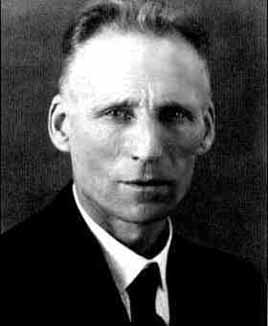
\includegraphics[width=\linewidth]{brouwer}
\caption*{Luitzen Brouwer}
\label{fig:test1}
\end{minipage}\hfill
\begin{minipage}{.3\textwidth}
\centering
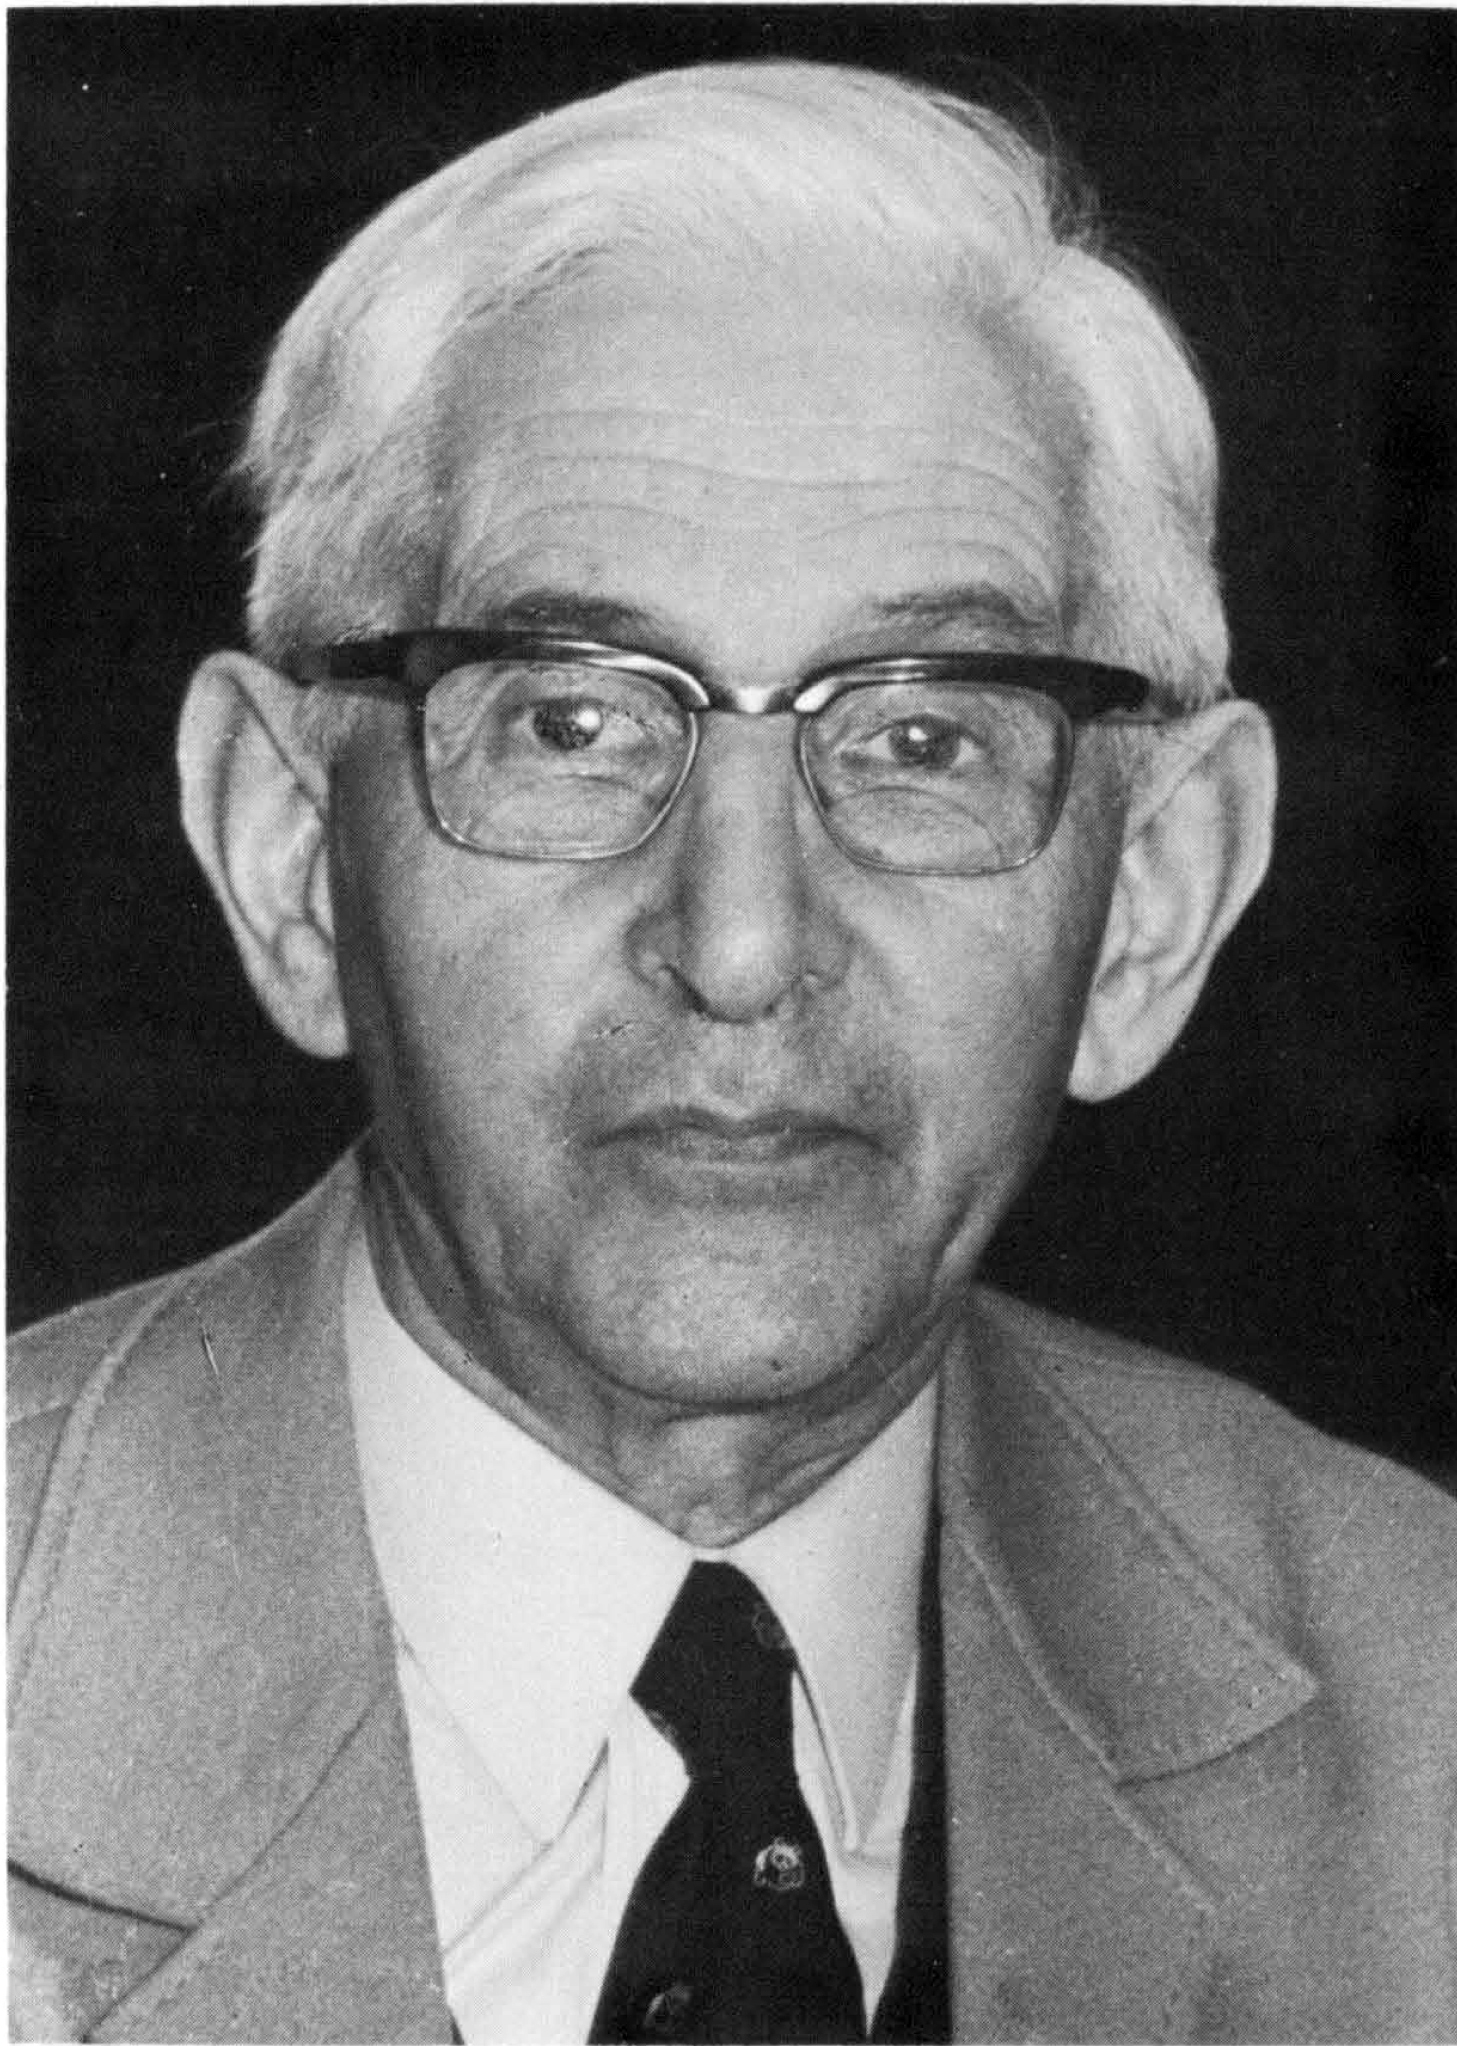
\includegraphics[width=\linewidth]{heyting}
\caption*{Arend Heyting}
\label{fig:test2}
\end{minipage}\hfill
\begin{minipage}{.3\textwidth}
\centering
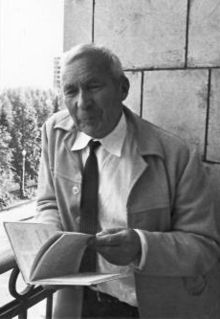
\includegraphics[width=\linewidth]{kolmogorov}
\caption*{Andrey Kolmogorov}
\label{fig:test3}
\end{minipage}
\end{figure}
  

\end{frame}

\begin{frame}
  \frametitle{BHK-interpretation}
  Brouwer-Heyting-Kolmogorov interpretation of logical constants
  \begin{itemize}
  \item A proof of $A \wedge B$ is a pair $(a, b)$ where $a$
    is a proof of $A$, and $b$ is a proof of $B$
  \item A proof of $A \vee B$ is a pair $(a, 1)$ where $a$
    is a proof of $A$, or a pair $(0, b)$ where $b$ is a proof of $B$
  \item A proof of $A \longrightarrow B$ is a function that takes
    proofs of $A$ as inputs and produces proofs of $B$ as outputs
  \item A proof of $\exists x \in A : \phi(x)$ is a pair
    $(a, b)$ where $a \in A$, b is a proof of $\phi(a)$
  \item A proof of $\forall x \in A : \phi(x)$ is a function
    $f : A \longrightarrow \Phi$, $a \mapsto \phi(a)$ that
    converts elements $a$ of $A$ into proofs $\phi(a)$
  \item Negation defined as $A \longrightarrow \bot$
  \item $\bot$ is an absurd statement ($2 = 3$) that cannot be proven
  \item * Ex Falso Quodlibet: $\bot \longrightarrow A$, where $A$ is arbitrary
  \end{itemize}
\end{frame}

\begin{frame}
  \frametitle{Curry-Howard isomorphism (propositions-as-types)}

\begin{center}
\begin{tabular}{ | c | c | }
  \hline
  Proof Theory & Type Theory \\ \hline
  Proposition $A$ & Type $А$ \\
  Proof of $А$ & $\Gamma \vdash a : A$ \\
  $ A \wedge B $ & Product A B \\
  $ A \vee B$ & Sum A B  \\
  $ A \supset B $ & $ A \rightarrow B $ \\
  $\neg A (i. e. A \rightarrow \bot)$ & $ A \rightarrow \bot$  \\
  true, false & $\top$, $\bot$  \\
  \hline
  $\forall x \in A . B(x)$ & $\prod_{x:a}^{} B(x)$  \\
  $\exists x \in A . B(x)$ & $\sum_{x:a}^{} B(x)$  \\
  \hline
  Induction & Inductive type (e.g. $\mathbb{N}$) \\
  \hline
  Pierce's law  & Continuation  \\
  $ ((P \rightarrow Q) \rightarrow P) \rightarrow P$ & \\
  \hline
  double-negation translation & Continuation-passing style \\
  \hline 
\end{tabular}
\end{center}
\end{frame}

\section{Interlude}

\begin{frame}
  \frametitle{Remarks}
  


    \begin{minipage}{.45\textwidth}
      \begin{itemize}
        \item de Bruijn principle
        \item MLTT
        \item Girard's Paradox
        \item HoTT
        \item Coq
        \item Agda
        \item Idris
        \item NuPRL
        \item Lean
        \item ...
      \end{itemize}
    \end{minipage}
    \begin{minipage}{.45\textwidth}
      \begin{center}
      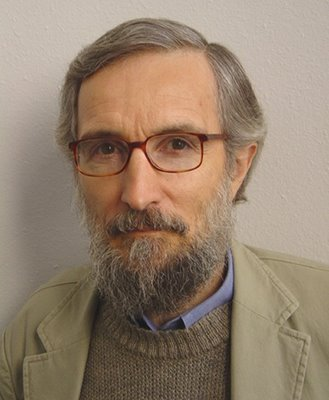
\includegraphics[scale=0.3]{Martinlof}
      \\ Per Martin-L\"of
      \end{center}
    \end{minipage}
\end{frame}



\section{Development}

\begin{frame}
  \frametitle{Plan}
  \begin{itemize}
  \item Theoretical basics ($\Pi$, $\Sigma$, $ac$, $\top$, $\bot$, $\equiv$, $\cong$)
  \item Types $\&$ theorems ($\mathbb{B}$, $\mathbb{N}$, List, Vector, Stream)
  \item Monoid, Functor, Monad
  \end{itemize}
\end{frame}

\section{MLTT}

\begin{frame}
\frametitle{$\Pi$ type}
\ExecuteMetaData[agdastuff/latex/MLTT.tex]{pi}
\end{frame}

\begin{frame}
\frametitle{$\Sigma$ type}
\ExecuteMetaData[agdastuff/latex/MLTT.tex]{sigma}
\end{frame}

\begin{frame}
\frametitle{Identity type}
\ExecuteMetaData[agdastuff/latex/MLTT.tex]{id}
\end{frame}

\begin{frame}
\frametitle{Logic}
\ExecuteMetaData[agdastuff/latex/MLTT.tex]{logic}
\end{frame}

\begin{frame}
\frametitle{Axiom of Choice}
\ExecuteMetaData[agdastuff/latex/MLTT.tex]{ac}
\end{frame}
\section{Booleans}

\begin{frame}
\frametitle{Booleans}
\ExecuteMetaData[agdastuff/latex/Bool.tex]{defbool}
\end{frame}

\begin{frame}
\frametitle{Operations on Booleans}
\ExecuteMetaData[agdastuff/latex/Bool.tex]{defops}
\end{frame}
 
\begin{frame}
\frametitle{Idempotence}
\ExecuteMetaData[agdastuff/latex/Bool.tex]{idemp}
\end{frame}
  
\begin{frame}
\frametitle{Distributivity}
\ExecuteMetaData[agdastuff/latex/Bool.tex]{distrib}
\end{frame}
 
\begin{frame}
\frametitle{Absorption}
\ExecuteMetaData[agdastuff/latex/Bool.tex]{absorp}
\end{frame}


\section{Natural Numbers}

\begin{frame}
\frametitle{Natural numbers}
\ExecuteMetaData[agdastuff/latex/Nats.tex]{natsdef}
\end{frame}

\begin{frame}
\frametitle{0 is right rero}
\ExecuteMetaData[agdastuff/latex/Nats.tex]{leftplus}
\end{frame}

\begin{frame}
\frametitle{+ commutes}
\ExecuteMetaData[agdastuff/latex/Nats.tex]{comm}
\end{frame}

\begin{frame}
\frametitle{* left distributive to +}
\ExecuteMetaData[agdastuff/latex/Nats.tex]{distr}
* Some auxiliary proofs are not shown
\end{frame}

\section{Lists}

\begin{frame}
\frametitle{Lists}
\ExecuteMetaData[agdastuff/latex/List.tex]{listdef}
\end{frame}

\begin{frame}
\frametitle{Functions on Lists}
\ExecuteMetaData[agdastuff/latex/List.tex]{funs}
\end{frame}

\begin{frame}
\frametitle{Second functor law}
\ExecuteMetaData[agdastuff/latex/List.tex]{functor}
\end{frame}

\begin{frame}
\frametitle{Reverse preserves length}
\ExecuteMetaData[agdastuff/latex/List.tex]{reverse}
\end{frame}

\section{Vector}

\begin{frame}
  \frametitle{Internal vs External}
  \begin{itemize}
  \item The way to reason about programs shown in previous examples is called
  \textbf{external} verification: we define non-dependent types and reason about them using $\equiv$.
\item Another way to produce verified programs is to define a
  \textbf{dependent familly of datatypes} along with their
  intrinsic properties, which make it impossible to produce incorrect programs.
  This side of verificationism is calles \textbf{internal} verification.
\item An familly $T$ of types indexed with \textbf{values}
  of another type $I$ means that for each $i:I$ we have a member of this type familly $T_i$.
\item For instance, a type familly indexed over $\mathbb{B}$ would have precisely two members.
\item A classic example of a dependent type is a dependent vector: a List-like container which can store a precise number of elements
\item In recent versions of haskell some "dependent types" can be simulated
  using type families and type-level programming
  \end{itemize}
  
\end{frame}

\begin{frame}
\frametitle{Vectors}
\ExecuteMetaData[agdastuff/latex/Vector.tex]{vecdef}
\end{frame}

\section{Coinduction}

\begin{frame}
\frametitle{Basic operations \& Streams}
\ExecuteMetaData[agdastuff/latex/Coind.tex]{imaginary}
\end{frame}

\begin{frame}
\frametitle{Some recursive functions}
\ExecuteMetaData[agdastuff/latex/Coind.tex]{rec}
\end{frame}


\begin{frame}
\frametitle{Some corecursive functions}
\ExecuteMetaData[agdastuff/latex/Coind.tex]{corec}
\end{frame}


\begin{frame}
\frametitle{Equivalence on streams}
\ExecuteMetaData[agdastuff/latex/Coind.tex]{equiv}
\end{frame}

\begin{frame}
\frametitle{Proofs about Stream equivalence}
\ExecuteMetaData[agdastuff/latex/Coind.tex]{proofs}
\end{frame}

\section{Monoids}

\begin{frame}
\frametitle{Monoids \& Instance arguments}
\ExecuteMetaData[agdastuff/latex/MonFunMon.tex]{monoid}
\end{frame}

\begin{frame}
\frametitle{Monoid \& Instance arguments}
\ExecuteMetaData[agdastuff/latex/MonFunMon.tex]{listmonoid}
\end{frame}

\section{Functors}

\begin{frame}
\frametitle{Functor}
\ExecuteMetaData[agdastuff/latex/MonFunMon.tex]{functor}
\end{frame}

\begin{frame}
\frametitle{List Functor}
\ExecuteMetaData[agdastuff/latex/MonFunMon.tex]{listfunctor}
\end{frame}

\section{Monads}

\begin{frame}
\frametitle{Monad}
\ExecuteMetaData[agdastuff/latex/MonFunMon.tex]{monad}
\end{frame}

\begin{frame}
\frametitle{Maybe Monad}
\ExecuteMetaData[agdastuff/latex/MonFunMon.tex]{maybemonad}
\end{frame}


\section{Finale}

\begin{frame}
  \frametitle{Symbols}
  \begin{center}
  \begin{tabular}{ | c | c | c | c | c | c | }
  \hline
    $\Pi$ & \texttt{\textbackslash Pi}
    & $\Sigma$ & \texttt{\textbackslash Sigma}
    & $\Sigma$ & \texttt{\textbackslash Sigma}
    \\  \hline
    $\ell$ & \texttt{\textbackslash ell}
    & $\lambda$ & \texttt{\textbackslash Gl}
    & $\Sigma$ & \texttt{\textbackslash Sigma}
    \\  \hline
    $\rightarrow$ & \texttt{\textbackslash r}
    & $\langle$ & \texttt{\textbackslash <}
    & $\Sigma$ & \texttt{\textbackslash Sigma}
    \\  \hline
    $\infty$ & \texttt{\textbackslash inf}
    & $\flat$ & \texttt{\textbackslash b}
    & $\Sigma$ & \texttt{\textbackslash Sigma}
    \\  \hline
    $\sharp$ & \texttt{\textbackslash \#}
    & $\mathbb{B}$ & \texttt{\textbackslash bb}
    & $\Sigma$ & \texttt{\textbackslash Sigma}
    \\  \hline
    $\mathbb{N}$ & \texttt{\textbackslash bn}
    & $\top$ & \texttt{\textbackslash top}
    & $\Sigma$ & \texttt{\textbackslash Sigma}
    \\  \hline
    $\bot$ & \texttt{\textbackslash bot}
    & $\equiv$ & \texttt{\textbackslash ==}
    & $\glb$ & \texttt{\textbackslash glb}
    \\  \hline
    $\cong$ & \texttt{2 tilda}
    & $::$ & \texttt{\textbackslash ::}
    & $\lub$ & \texttt{\textbackslash lub}
    \\  \hline
    $\oplus$ & \texttt{\textbackslash oplus}
    & $\otimes$ & \texttt{\textbackslash otimes}
    & $\mapsto$ & \texttt{\textbackslash mapsto}
    \\  \hline
    $\circ$ & \texttt{\textbackslash o}
    & $\omega$ & \texttt{\textbackslash om}
    & $\Omega$ & \texttt{\textbackslash Omega}
    \\  \hline 
  \end{tabular}
  \\ \\ * To find out how to type arbitrary symbol,
  \\ use \texttt{M-x describe-char} in Agda mode.
  \end{center}
\end{frame}

%\begin{frame}
%  \frametitle{Shortcuts}
%  \begin{center}
%  \begin{tabular}{ | c | c | c | c | c | c | }
%  \hline
%     A & B
%    & C & D
%    & E & F
%    \\ \hline
%     A & B
%    & C & D
%    & E & F
%    \\ \hline
%     A & B
%    & C & D
%    & E & F
%    \\ \hline
%     A & B
%    & C & D
%    & E & F
%    \\ \hline
%     A & B
%    & C & D
%    & E & F
%    \\ \hline
%     A & B
%    & C & D
%    & E & F
%    \\ \hline
%     A & B
%    & C & D
%    & E & F
%    \\ \hline
%     A & B
%    & C & D
%    & E & F
%    \\ \hline
%    
%  
%\end{tabular}
%\end{center}
% \end{frame}

\begin{frame}
  \frametitle{Resources}
  \begin{itemize}
  \item A bit outdated: \url{http://oxij.org/note/BrutalDepTypes/}
  \item Wiki: \url{http://wiki.portal.chalmers.se/agda}
  \item Classic tutorial: \\ \url{www.cse.chalmers.se/~ulfn/papers/afp08/tutorial.pdf}
  \item \url{http://www.cse.chalmers.se/~peterd/papers/DependentTypesAtWork.pdf}
  \item Wonderfull tutorial here \\ \url{http://people.inf.elte.hu/divip/AgdaTutorial/Index.html}
  \item Norell's PhD
  \item Agda Standard Library \\ \url{https://github.com/agda/agda-stdlib}
  \item NAL (NURE Agda Library) \\ \url{https://github.com/zelinskiy/NAL}
  \end{itemize}
\end{frame}

\begin{frame}
  \frametitle{Books}
  \begin{figure}[ht] 
  \label{ fig7} 
  \begin{minipage}[b]{0.5\linewidth}
    \centering
    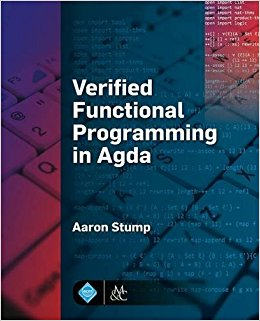
\includegraphics[width=.3\linewidth]{agdabook} 
    \caption*{A. Stump} 
    \vspace{4ex}
  \end{minipage}%%
  \begin{minipage}[b]{0.5\linewidth}
    \centering
    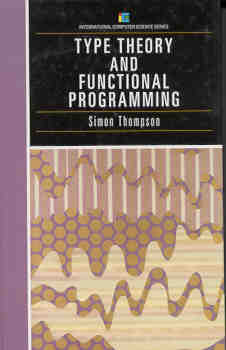
\includegraphics[width=.3\linewidth]{ttfpbook} 
    \caption*{S. Thompson} 
    \vspace{4ex}
  \end{minipage} 
  \begin{minipage}[b]{0.5\linewidth}
    \centering
    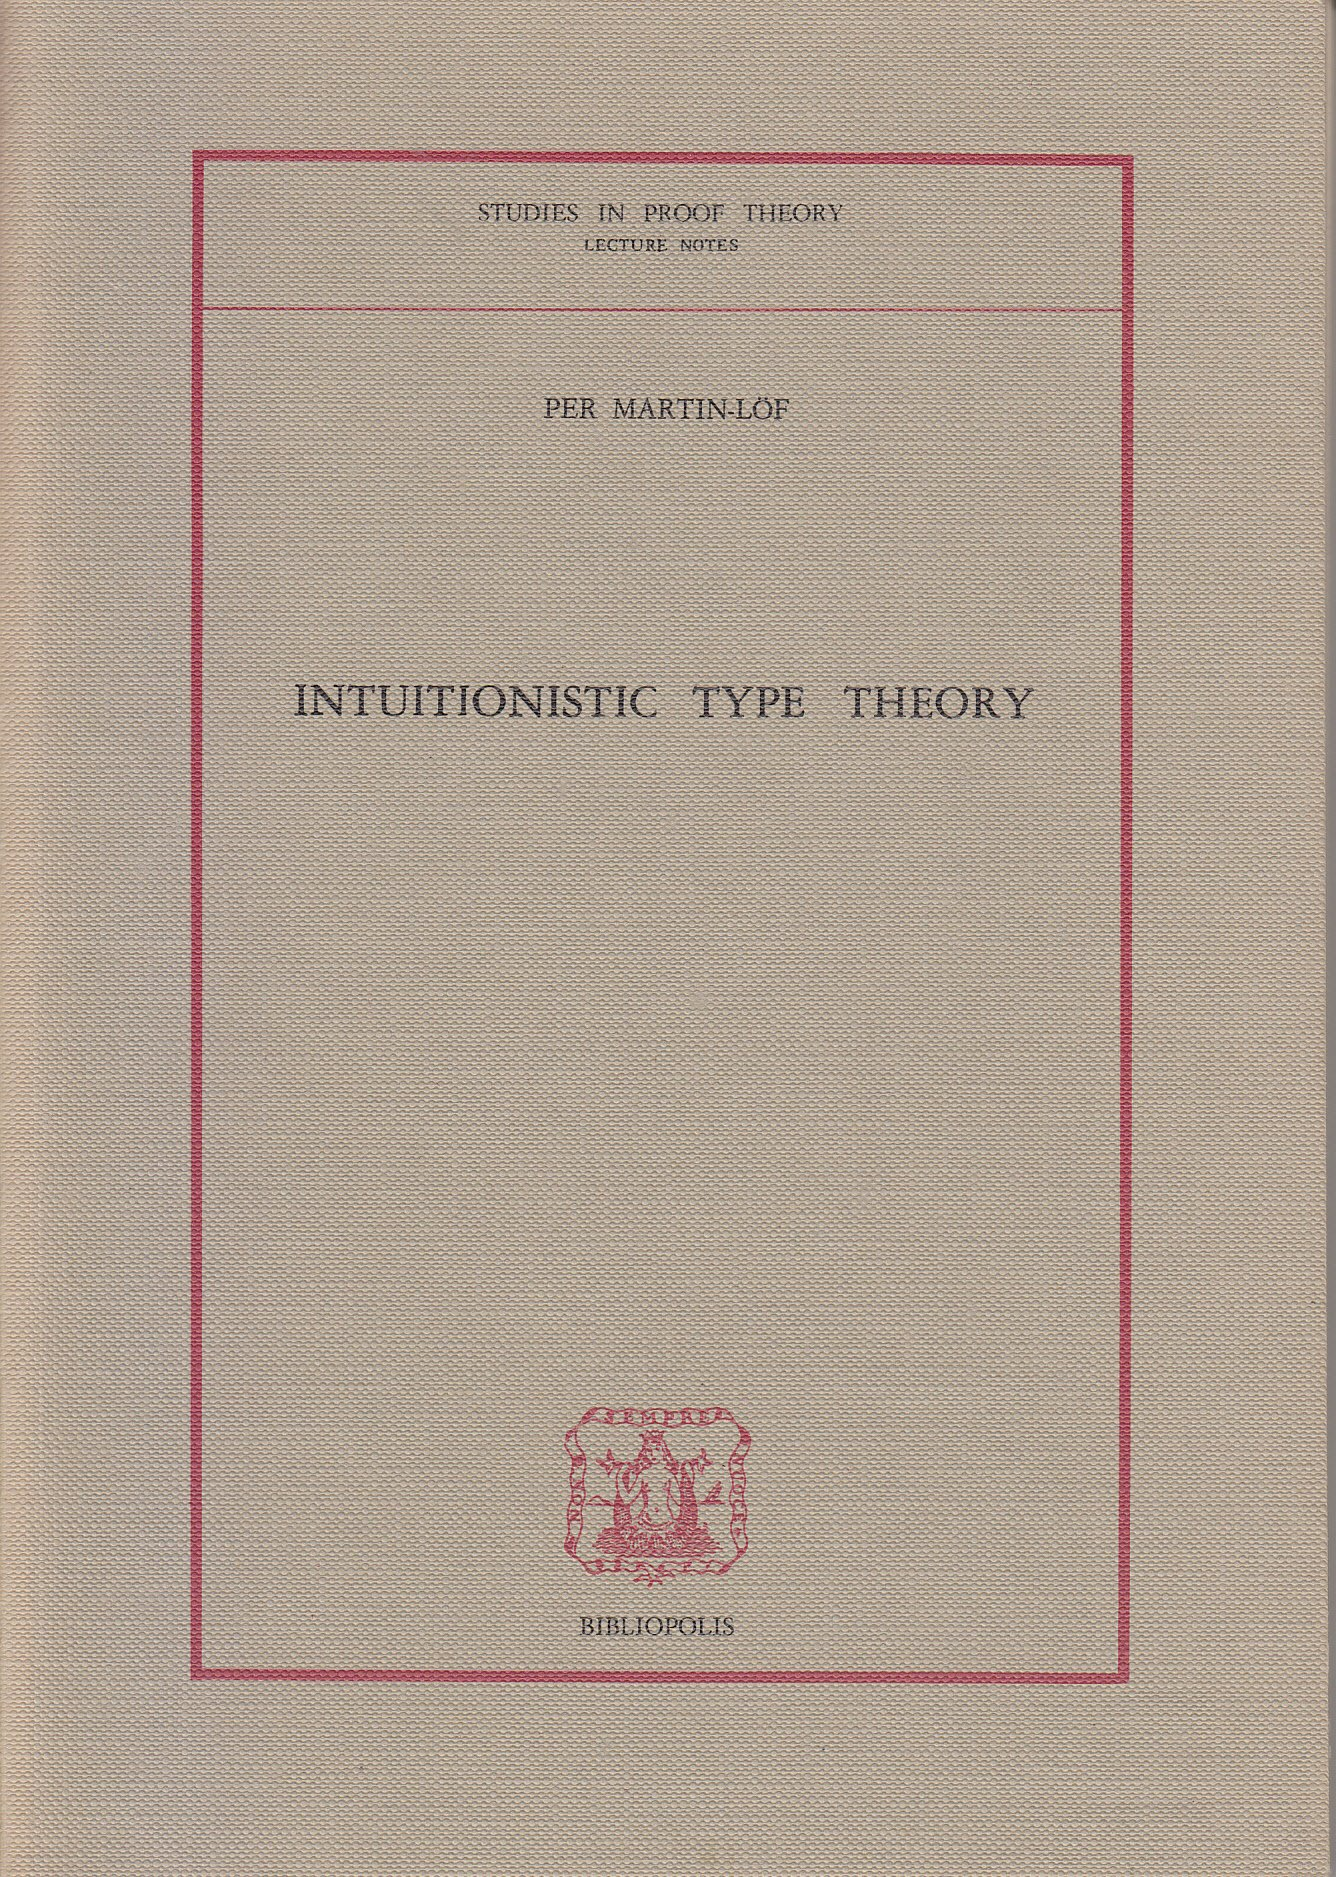
\includegraphics[width=.3\linewidth]{mlttbook} 
    \caption*{P. Martin-L\"of} 
    \vspace{4ex}
  \end{minipage}%% 
  \begin{minipage}[b]{0.5\linewidth}
    \centering
    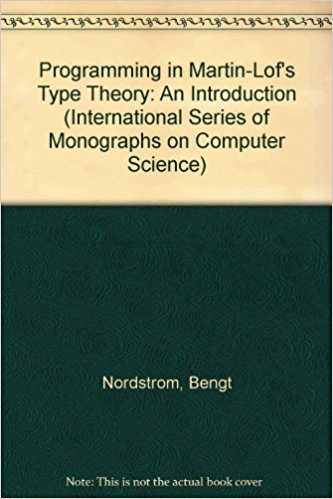
\includegraphics[width=.3\linewidth]{nordstrombook} 
    \caption*{B. Nordstr\"om} 
    \vspace{4ex}
  \end{minipage} 
\end{figure}
\end{frame}

\section{Questions}

\end{document}